\chapter{Introduction: Robots, Interaction and Knowledge}
\label{chapt|introduction}


This shift requires ``awareness'' of humans.

To make informed decision, the robot needs knowledge about the \emph{tasks},
the \emph{environment}, the \emph{situational context}.
%%%%%%%%%%%%%%%%%%%%%%%%%%%%%%%%%%%%%%%%%%%%%%%%%%%%%%%%%%%%%%%%%%%%%%%%%%%%%%%

List of recent successful \& highly visible robot experiments in human environment:
\begin{itemize}
    \item Amener une bierre avec le PR2 (WG)
    \item Sandwiches/popcorn at TUM
    \item expe avec Nao
\end{itemize}

Service robotics is leaving the realm of Sci-Fi, dreams and fanstasms to become
a reality. \fxwarning{find references of predictions "when robots are in our
homes}. 

Robotics is moving from technological demos to real world coworkers/companions.


Decision making on the robot can not anymore rely on a single or a few
modalities of interaction.

The perceptual layer has moved up from traditional sensing modalities (camera
images, laser scans) to synthetic pseudo-sensors like the Kinect-based human
tracker, face recognition or SLAM-based localization.

Perceiving and understanding the environment is nowadays mainly a matter of
rebuilding an internal, amodal, model of the environment with two interleaved
facets: a continuous, geometric world and a discrete, symbolic world.

But perceiving an inanimate environment is not enough: our robots do not live
anymore in isolation in a world that is tailored to their capabilities. They
live in the real world, in interaction with other intelligent agents. We want
them to be endowed with \emph{agency} (the ability to \emph{act} in the world)
and \emph{social skills}. This implies that the robot is not only able to
represent inanimate objects, not only able to represent its own mental state,
but also mental states of other agents, other intelligences. And interaction
also require communication skills, and social capabilities like perspective
taking or a theory of mind. Our robots also come to life in a connected world:
the interactions take place with other physical as well as disembodied agents.

Figure~\ref{fig|cognitive-robots} proposes an organization of research fields
and projects in robotics along two dimensions, the level of social skills, and
the level of agency (the ability to \emph{act in the world}).

\begin{figure}
    \centering
    
\includegraphics[width=0.7\columnwidth]{intro/social_skills.pdf}
    \caption{Towards the cognitive robot}
    \label{fig|cognitive-robots}
\end{figure}



\begin{itemize}
    \item to loosen the constraints on symbolic modeling of the robot
    environment by providing more expressive representation system than
    classical databases or fact repositories,

    \item to improve human-robot interaction by explicitly providing to the
    machine an interpretation frame, at least partially shared with the human.

\end{itemize}


%%%%%%%%%%%%%%%%%%%%%%%%%%%%%%%%%%%%%%%%%%%%%%%%%%%%%%%%%%%%%%%%%%%%%%%%%%%%%%%
%%%%%%%%%%%%%%%%%%%%%%%%%%%%%%%%%%%%%%%%%%%%%%%%%%%%%%%%%%%%%%%%%%%%%%%%%%%%%%%
%%%%%%%%%%%%%%%%%%%%%%%%%%%%%%%%%%%%%%%%%%%%%%%%%%%%%%%%%%%%%%%%%%%%%%%%%%%%%%%

\section{A prototypical scenario}
\label{sect|scenario}

\begin{figure*}
	\centering
	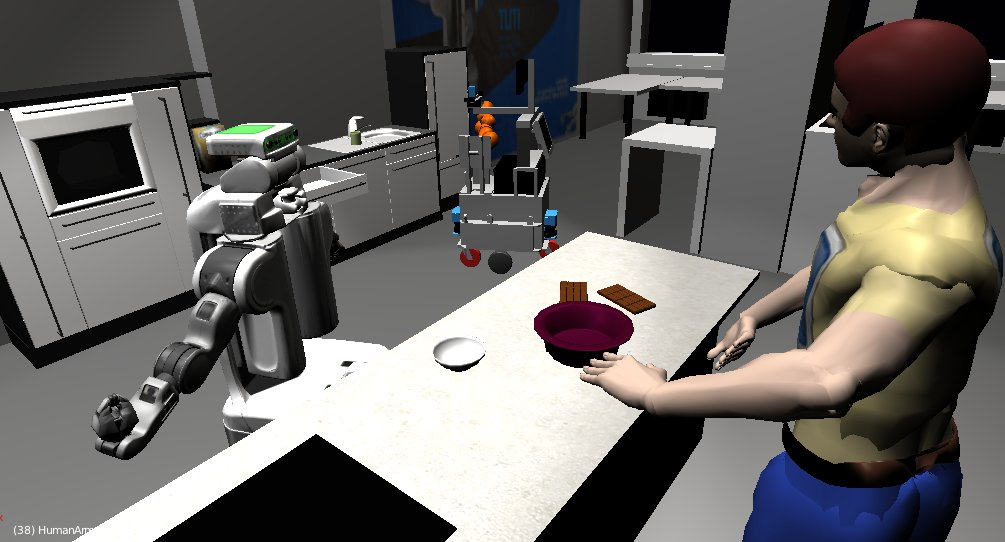
\includegraphics[width=0.9\textwidth]{intro/brownie_scenario.jpg}
	\caption{An illustration of the scenario}
	\label{fig|scenario}
\end{figure*}

The aim of this imaginary scenario (that has not been implemented, neither in
simulation nor on a robot) is to materialise early in this thesis the context
and challenges of knowledge representation and manipulation for service, social
and interactive robotics. It underlines the place, the role and the need of
knowledge in a near-future, everyday situation where several robots and humans
co-exist and cooperate. This scenario will also be a source of support examples
for later sections of the thesis.

We entitle our scenario ``the Brownie scenario'' (Figure~\ref{fig|scenario}):
Robi and Roba are two service robots, that can freely
move and pick objects around (with possibly different hardware and softwares
architectures, including different knowledge representation systems). They
cooperate with a human in a kitchen environment.

The main task of the scenario is the joint realization of a brownie, initiated
by Tom, the human: ``Let's make a brownie for tonight!''.

The scenario is successful if the task is achieved (the brownie is baked) in a
reasonable time (typically shorter than what it would have been required by the
human alone).

We voluntarily do not detail the subtasks of the scenario, neither we define
how they are shared amongst agents: our focus is on knowledge needs and flows.

A ``first-order'' analysis of this task leads to a rough partition of the
required \emph{representation} abilities:

\begin{enumerate}

	\item Representation abilities related to the execution of a complex
	spatio-temporal task,

	\item Representation abilities related to cooperation with other agents.

\end{enumerate}

% Representation of a complex task
We can further refine these categories: to prepare and bake a brownie, the
robot first needs to make sense of the term \emph{brownie} itself: what is it?
what is it used for? what is it made of? etc. We call this knowledge
\emph{common-sense knowledge} and the robot must be able not only to represent
it, but also to have access to an initial source (for instance through a
initial set of facts that are made available at startup, or via access to a
Web-based knowledge base like Wikipedia, etc.)

Once bound to the action \emph{make}, this should lead the robot to build and
represent a \emph{context}: we are in a scenario involving cooking. The context
enables the robot to retrieve more common-sense knowledge, like that actions
related to cooking often take place in the kitchen, cooking requires
ingredients, utensils and a procedure that may be provided by a recipe.

These last assertions imply several other capabilities: ``cooking often takes
place in the kitchen'' implies that representation of both uncertainty and
likelihood is desirable. The fact that cooking is associated to a place further
implies that the system models locations and is able to attach \emph{thematic
relations} to concepts (here, the likely location of the cooking action).

``cooking requires ingredients'' hints about another important feature closely
tied on knowledge manipulation: \emph{reasoning}. The robot can \emph{infers}
that cooking may require a recipe since a list of ingredients is a
pre-requisite of the cooking action, and a recipe may provide such a list.  If
we omit the ``may'', this is a typical example of first-order logic reasoning.
Many other reasoning techniques exist (including probabilistic ones -- ones
able to deal with the ``may''), we shall illustrate some of them later in this
scenario.

We mentioned that a recipe often provides a procedure (or a \emph{plan}). The
robot should be able to store this plan in a way that allow later execution.
The plan is likely to contain \emph{spatio-temporal constraints} (like ``put
the brownie in the oven for 20 min'' or ``let's cook \emph{for tonight}'') that
must be as well appropriately handled.

To make decision, a robot may also want to \emph{predict} the state of the
world after some action (``if I leave the cake 2h in the oven, it will burn'').
Such ability to project itself in future or, generally speaking, in other
possible state of the world is related to several cognitive ability and
reasoning techniques: \emph{planning}, \emph{projection}, \emph{representation
of possible worlds} and \emph{non-monotonic reasoning}, in addition to
common-sense knowledge and \emph{physics-based} reasoning (that allows for
instance to predict that an egg is likely to break if dropped).

Procedures are in addition often \emph{underspecified}: we can expect the
recipe to provide a cooking duration, but we usually do not expect the recipe
to tell us to first open the oven door, and then put the cake into it, since it
is self-evident that the door must first be opened to put the cake in the oven.
Our cognitive robot should ideally be able to detect and possibly complete such
underspecification.

% Representation feature that enable cooperation
Then, we want our three agents to cooperate. This, in turn, leads to another
set of cognitive abilities.

Cooperation in our scenario can intervene at many places. For instance, an
agent may want to inform another one about the number of eggs that are
necessary for the brownie. This \emph{helping} behaviour makes sense only if
the first agent knows that the recipient agent both needs the information but
does not know it. This in turn requires the robot to be able to model the
knowledge of the other agents: to think \emph{from the perspective} of another
agent (an idea that is related to the availability of a theory of mind, we will
come back to it later on).

Ability to communicate is one important pre-requisite to collaboration.
Communication in general requires the addresser and the addressee to share a
common interpretative framework (a shared common-sense knowledge -- or cultural
background -- and a shared context). In our scenario, the agents are working in
a kitchen. This element of context does not however suffice if, for example, an
agent asks another agent to ``give {[him]} the bowl''. Behind the symbol
``bowl'', which physical entity are we actually talking about? If we want to
talk and act on the world, this so-called \emph{grounding} operation is
essential. It is a bidirectional process: in covers the {\it top-down}
operation (from the symbol to the percept) and the {\it bottom-up} converse
(retrieval or creation of symbols from perception).

A related ability is called \emph{pre-supposition accommodation}: if one of the
agent moves behind another one, with the brownie dough in its arm, and says
``be careful, I'm behind you!'', we want the first agent to be able to
represent both symbolically and geometrically (because, for instance, if the
agent want to move, it must take into account the new obstacle) something that
is not directly perceived.

Also central to cooperation are the notions of \emph{joint intentions} and
\emph{joint goals}: to help the human during the cooking session, the robots
need to track how far they are into the recipe, what is the next step the human
is likely to go for, how task are currently split between agents, what action
is currently blocking the procedure, etc. This knowledge should let the robot
identify the intentions of other agents and create accordingly joint goals.
Hence, a knowledge representation system aiming at dealing with cooperative
behaviours is likely to have goal management structures taking explicitly into
account other agents' actions and goals.

In order to effectively share tasks, the robot must also know what it is
capable of: \emph{capability introspection} (both in term of general capability
and of immediate ability) is thus often desirable. It can be extended to
general introspection (like the ability to tell ``who I am'' or ``what do I
think of'') that may be required for the interaction.

Last but not least, our scenario assumes implicitly \emph{natural interaction}
between humans and robots (as showed by the casual style of the order ``Let's
make a brownie!''), and we want to ensure that the
knowledge available to the robot provides efficient support to the natural
language understanding (for instance by adopting models and vocabulary that are
both well suited for machine processing and remain as close as possible to the
humans own structures and vocabulary), and also to \emph{non-verbal forms of
communication}, like gestures.


We have emphasised several keywords in this scenario: we will come back to them
in chapter~\ref{chapt|krs} to explain them formally, and relate them to each
other. Before that, we would like to briefly focus on the challenges
specifically related to the human-robot interactions. Not only in term of
knowledge representation, but more broadly in term of specific cognitive
capabilities.

%%%%%%%%%%%%%%%%%%%%%%%%%%%%%%%%%%%%%%%%%%%%%%%%%%%%%%%%%%%%%%%%%%%%%%%%%%%%%%%
%%%%%%%%%%%%%%%%%%%%%%%%%%%%%%%%%%%%%%%%%%%%%%%%%%%%%%%%%%%%%%%%%%%%%%%%%%%%%%%
%%%%%%%%%%%%%%%%%%%%%%%%%%%%%%%%%%%%%%%%%%%%%%%%%%%%%%%%%%%%%%%%%%%%%%%%%%%%%%%

\section{Robots for interaction}
\label{sect|hri-context}

This work comes indeed from researches in the specific context of the
human-robot interaction, or, to put it another way, in the context of
interaction for \emph{joint action} with human,  in a \emph{situated}
environment (figure~\ref{fig|aperitif}).

\begin{figure}%[!ht] 
    \centering
    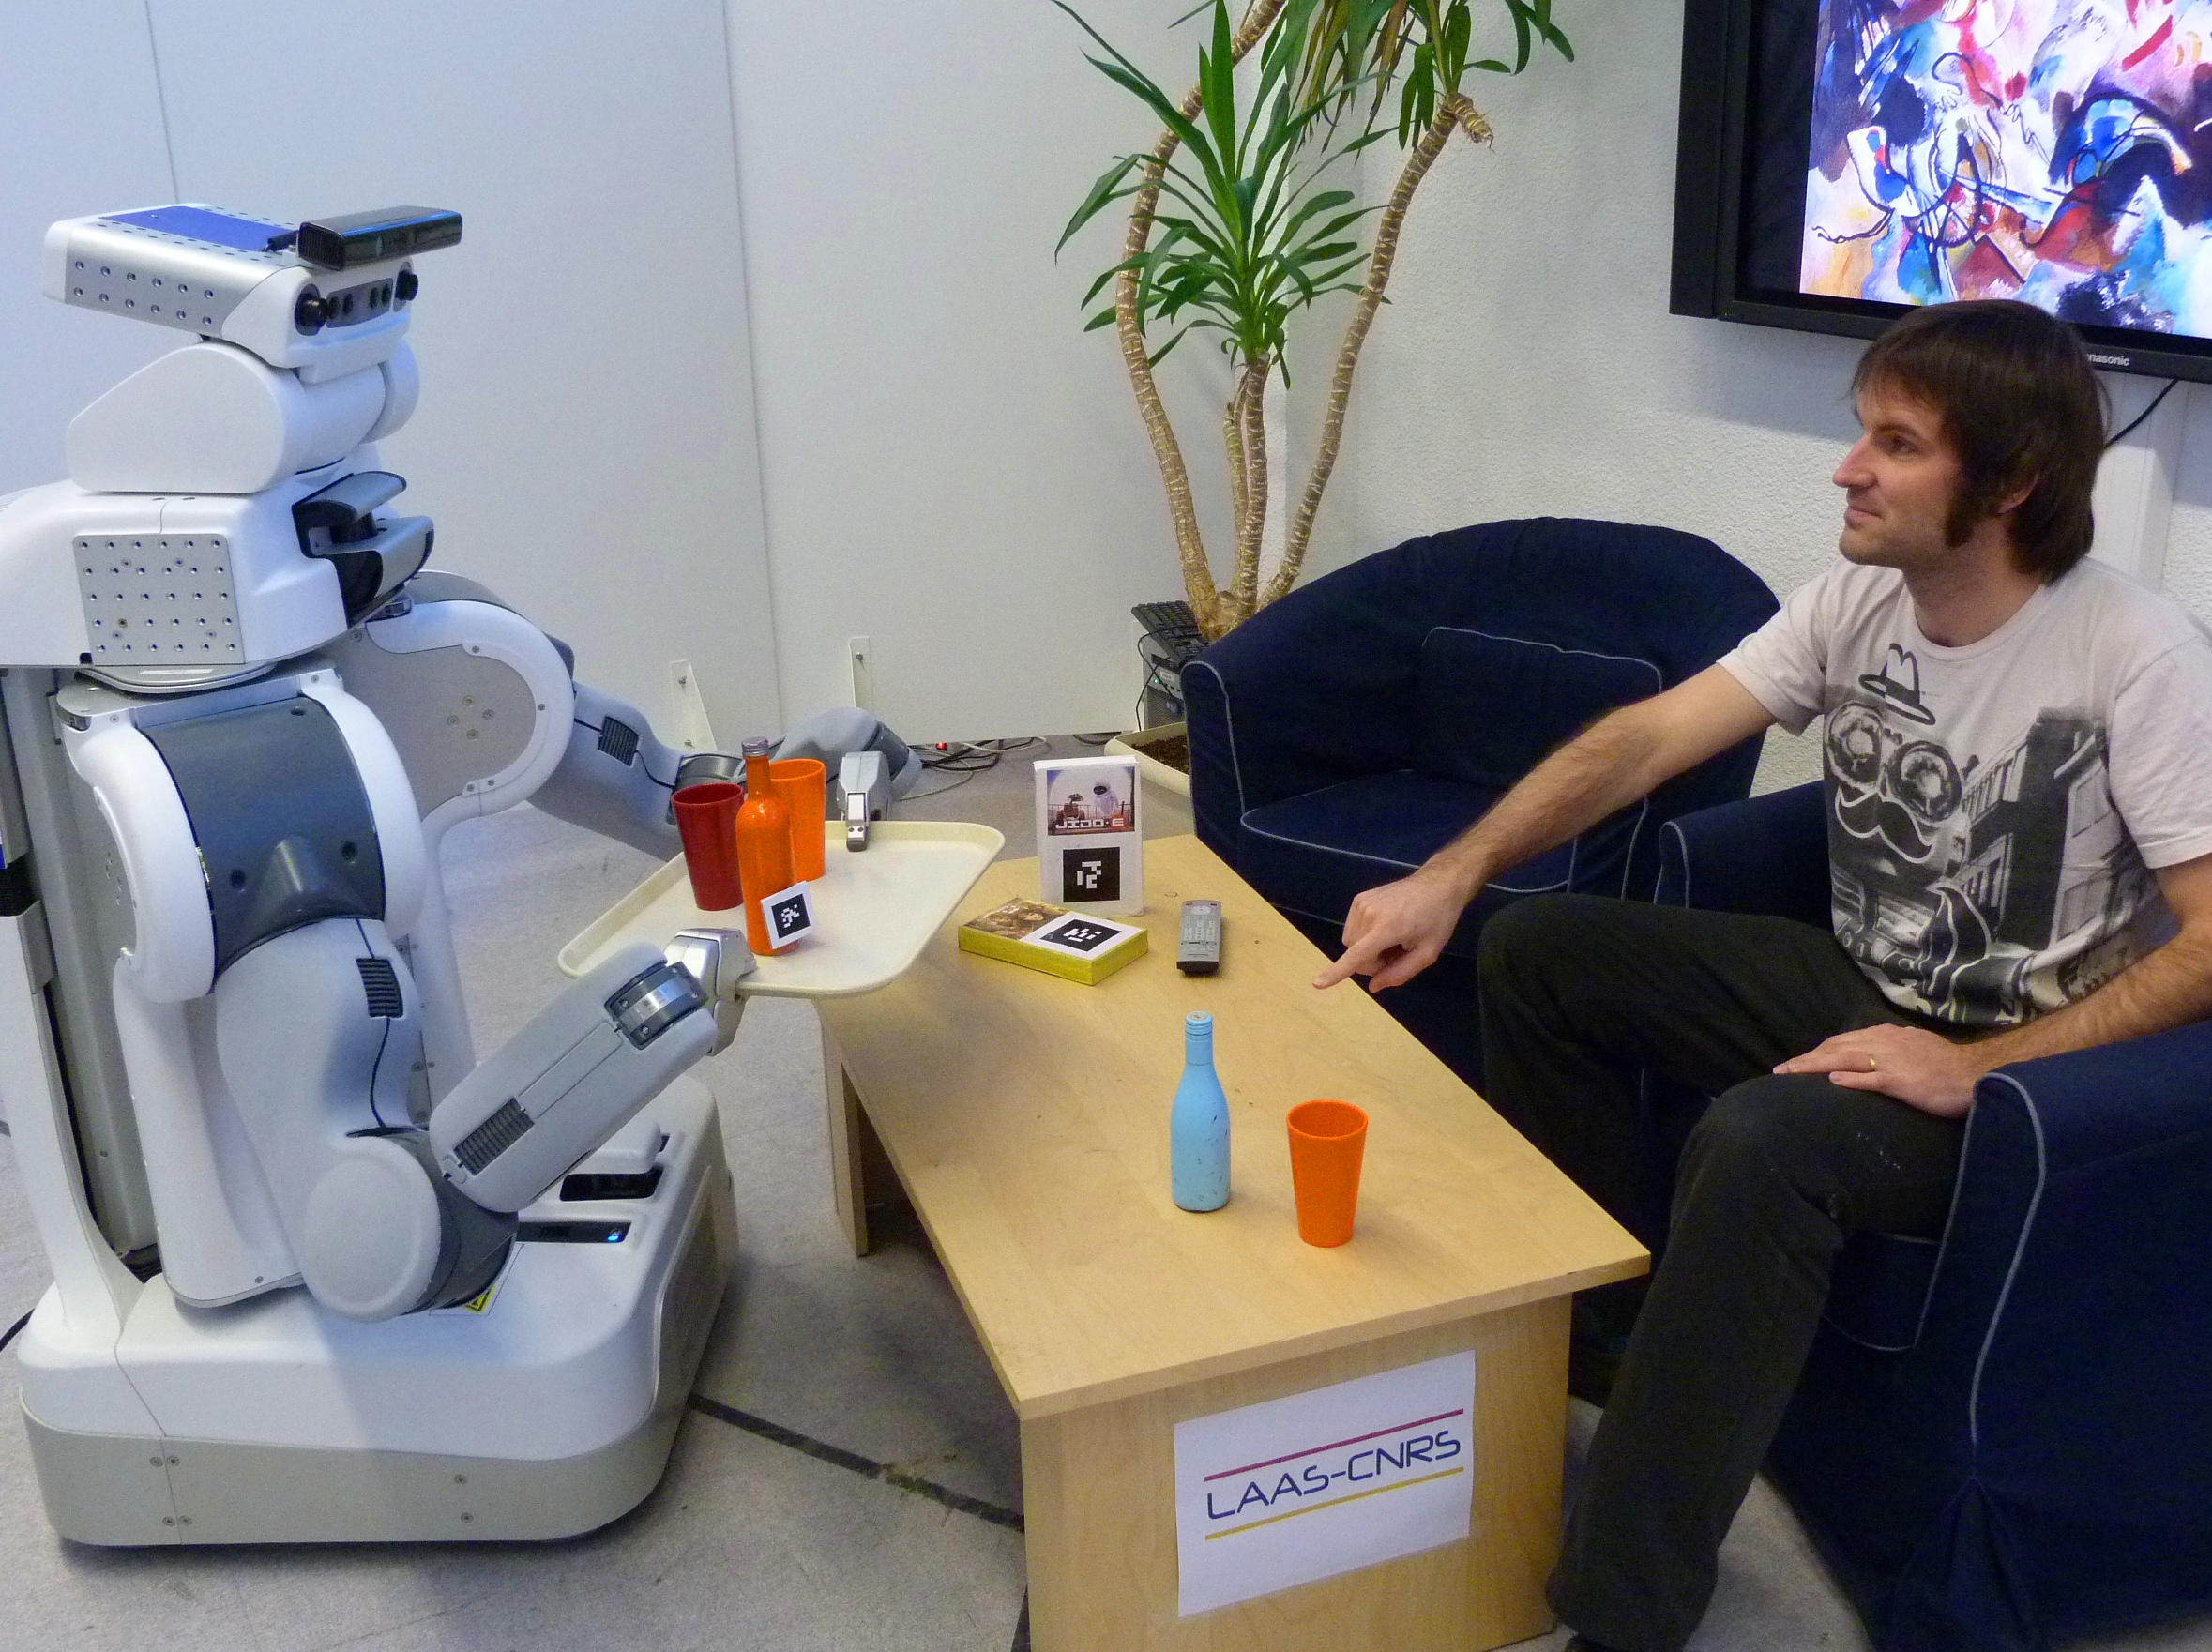
\includegraphics[width=0.8\columnwidth]{intro/aperitif_time.jpg} 

    \caption{Interacting with the robot in an everyday situation: the human
    asks for help in vague terms, the robot takes into account the human's {\it
    a priori} knowledge and spatial perspective to refine its understanding of
    the question.} 

    \label{fig|aperitif} 
\end{figure}

{\em \emph{Let's bake a brownie for tonight!}, proposes Tom. The robots
smoothly prepare all the ingredients, and they start to cook together a
delicious cake...}

Natural interaction and cooperation are actually the current (dare we say,
\emph{short-term}) targets for the human-robot interaction community.  The
``Brownie scenario'' we presented above belongs to the broad class of
\emph{interactive manipulation problems}: several agents agree on a (more or
less implicit) joint goal that requires some sort of cooperation to be
successfully achieved. This class of problems involves both dialogue and
manipulation and is often not completely defined at start-up: it requires
iterative, interactive resolution (step-by-step process,
questions-answers,...).

What are the cognitive prerequisites for such a sentence --``Let's make a
brownie for tonight''-- to be understood by the robot, correctly interpreted in
the spatial and temporal context of the interaction, and eventually transformed
into a set of actions? We distinguish~\cite{Lemaignan2012} four successive
steps:

\begin{enumerate}

    \item how to build and maintain a consistent geometric model of the current
        situation, acquired through perception or deduction from previous
        perceptions,

    \item how to build an unambiguous symbolic representation of concepts
        (objects, agents, actions...) underlying the interaction, and practical
        for decision-making processes,

    \item how to establish the joint goal(s), how to build and maintain
        iteratively shared (human-robot) plans, 

    \item how to refine and execute the computed plans, and how to monitor
        those achieved by its human partner?

\end{enumerate}

This work focuses on the second point: it presents techniques, developed and
used on several real robots, for the symbolic representation of environment
models suitable for grounded situation interpretation, decision-making and
control.

The other items are of course equally important to actually perform the
interaction, and we will also present (and illustrate in experiments) how our
knowledge representation system integrates and communicates with other
processes to form a \emph{knowledge-enabled} robotic architecture.


\begin{figure}
    \centering
    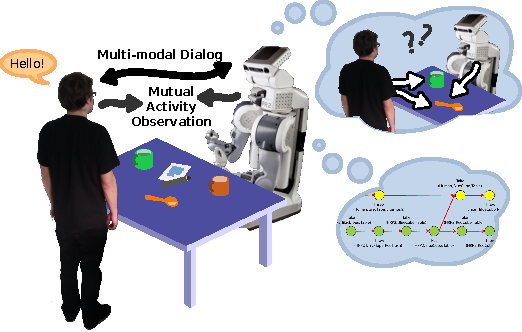
\includegraphics[width=0.9\columnwidth]{intro/grounding_robot.pdf}
    \caption{A robot reasoning about human-robot interaction and anticipation
    of human activities: sources of knowledge are multi-modal dialogue and
    observation of the environment and the human activities.}
    \label{fig|hri-dec}
\end{figure}


Figure~\ref{fig|hri-dec} summarises the main aspects of the interaction.
From the robot perspective, several cognitive skills are involved: dialogue
processing through verbal and deictic modalities (what does the human say? What
attitude -- glances, postures, gestures... -- does he express?), acquisition
and maintenance of one or several models of the environment, not only from the
robot point of view, but also from the other agents' points of view,
anticipation (what are the intentions of the human? Can I predict and
anticipate his/her actions?), planning and control (how would I proceed further
towards the goal?), monitoring of the other agents' activities (do we have an
effective cooperation?) and the overall progress of the task. 

As we shall see, all these cognitive capabilities also translate into
requirements on the knowledge representation systems that we want to clarify.

\begin{figure}%[!ht]
\centering
  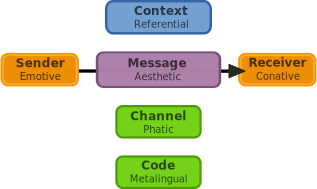
\includegraphics[width=0.6\linewidth]{communication/jakobson_communication_model.pdf}

  \caption{The \emph{Communication Model}, as proposed by
  Jakobson~\cite{Jakobson1960}. In bold characters are the \emph{communication
  dimensions}, in italics, the corresponding \emph{communication functions}.}
  
  \label{fig|jakobson_communication_model}
\end{figure}


The need of communication is probably the most salient one. The classical model
of communication proposed by Jakobson in 1960
(figure~\ref{fig|jakobson_communication_model}) exposes in a bright way the
main functions involved in a communication, be it verbal or non-verbal. While
the \emph{channel} and the \emph{code} are the technical side of the
communication, the \emph{message} in relation with the \emph{context} are
directly concerned with the question of the \emph{meaning} which itself as
tight links with the knowledge available to the agent.

The question of the communication between a robot and another agent (in a broad
way: another robot, an human, but also a remote knowledge base or the robot's
developer) underlies many of the challenges of knowledge representation: how to
represent the knowledge I want to exchange, and how to recognize, represent and
share a context that ensures both the end of the communication channel
correctly interpret the message. Or, to put it another way: how to ensure the
\emph{meaning} is correctly carried around while conducting social
interactions.

%%%%%%%%%%%%%%%%%%%%%%%%%%%%%%%%%%%%%%%%%%%%%%%%%%%%%%%%%%%%%%%%%%%%%%%%%%%%%%%

\section{The Challenges}
\label{sect|challenges}

From the set of questions raised in the previous paragraphs, we can now
articulate the challenges that are to be tackled in this field of knowledge
representation for service/companion robotics.

The first challenge is to... clarify the challenges (!) of knowledge
representation: we say ``knowledge'', we say ``reasoning'', we say
``representation'', but clear definitions are yet to be provided. Numerous
requirements on what Newell calls the \emph{knowledge level} of intelligent
agents have emerged from our \emph{Brownie} scenario, but how do they
articulate? And are they comprehensive?

To further develop what is widely known as the ``cognitive robotics'', we think
it is mandatory to lay down solid theoretical and practical foundations to the
knowledge needs of service/interactive robots. This is our first challenge.

The second challenge is more technical: how to build such a
``knowledge-enabled'' robot? Since many years, research has started to create
and study so-called cognitive architectures. Robots, as embodied and
interactive agents, raise specific issues. What are they? Which are the right
technical approaches? Can we build today such a cognitive system, and if we can
not, why that? How the abstract idea of knowledge translates into  practical,
meaningful concepts?

Our third challenge relates to the specific question of the human-robot
interaction: the robot enters the realm of a social individuality. What does
that mean? Which consequences does that have on our initial knowledge
challenge? How does it translate into practical issues, like natural language
understanding?

All the contributions (summarised in the next section) of this thesis can be
related to one of these three challenges, and hopefully contribute to the
advancement of the understanding of these questions.

%%%%%%%%%%%%%%%%%%%%%%%%%%%%%%%%%%%%%%%%%%%%%%%%%%%%%%%%%%%%%%%%%%%%%%%%%%%%%%%


\section{Contributions}
\label{sect|contributions}

We have presented our challenges: this section now summarises the main
contributions of the thesis, both from a scientific point of view and from a
technical point of view.

\subsection{Scientific contributions}
\label{sect|scientific-contributions}

The need of a better understanding of the knowledge needs of robotic
applications in human, \ie complex, dynamic, semantically-rich, environments,
is the starting point of our thesis.

Building upon an extensive review of the literature and the formulation of
several interaction scenarii (that themselves led to experiments on real
robots), we have iteratively refined the ``knowledge for interaction'' problem.
The formalization of this question is one of the main scientific outcomes of
this work: we have listed and organized into a typology a set of desirable
characteristics of knowledge representation systems for service robotics.

This typology aims at offering a comprehensive and consistent base to evaluate
existing systems and to draw new research perspectives. It also enables to
better assess the progresses of the Service Robot and Human Robot Interaction
research communities towards the long term goal of \emph{human-level artificial
intelligence} for robots, as would say McCarthy.

Another scientific contribution of this thesis is its participation to
narrow down the gap between research on embodied and disembodied artificial
agents: we have tried to bridge experiences learned from years of research on
disembodied cognitive architectures (both from the computing science and
neuropsychology communities) with the constraints from real-world systems that
weigh on robotic architectures. Notably, we have tried to identify
theoretical reference contributions from the diverse fields of cognitive
sciences that are relevant to \emph{knowledge-enabled} robotics. We have also
proposed reference implementations on robots for some of them.

At the architectural level, our work also helps to better understand the
knowledge flows in modern cognitive architectures for robots. By introducing
\emph{explicit} knowledge in our architectures, it allows the humans that
design and program robots to \emph{talk about} and question this knowledge: it
singularises and materialises concepts that were beforehand often
diffuse and ubiquitous. This leads us to define the idea and propose an
implementation of a \emph{knowledge-oriented} architecture.

This work has also several more focused scientific contributions. The
centralized semantic architecture that we propose is original. While it
exhibits shortcomings for some cognitive tasks, it also proposes novel efficient
ways to represent and manipulate knowledge simultaneously for multiple agents.
Along with the survey of current knowledge systems that we have conducted,
it effectively completes the panorama of available designs of knowledge
representation systems.

Amongst the cognitive abilities that our developments have enabled, a
particular scientific focus was led on the acquisition and modeling of
multiple, agent-dependent symbolic worlds. This opened new perspectives related
to \emph{perspective-aware} reasoning or \emph{theories of mind} for robots
that are detailed in this work.

We also have a scientific contribution on the grounding of human-robot
dialogue in natural language. We have algorithmically formalized a novel
grounding process that takes advantage of multi-modal communication (verbal,
deictic and immanent) and handles the semantics of several more complex
language features like quantification. This system also has contributions
related to the semantic validation of thematic roles and interactive
disambiguation that takes into account human attentional focus.

\subsection{Technical contributions}
\label{sect|technical-contributions}


This thesis has four major technical contributions: the software development of
\emph{ORO server} as a semantic blackboard dedicated to robotic applications,
the design of the \emph{ORO ontology} as a domain-specific common-sense
ontology tailored for service robotic needs, the pervasive integration of a new
semantic layer into several existing robot architecture, and finally, the
software development of \emph{Dialogs}, a novel module for natural language
grounding.

The main software contribution of the thesis is the development of an
open-source, versatile and light-weight knowledge base that stores in a
formal framework based on first-order logics both the robot's own beliefs and
the mental models of every other cognitive agents that the robot interacts
with. This tool, called \emph{ORO}, is implemented as a
platform/middleware-agnostic server, and exposes to the robot's modules
several advanced reasoning services (via the integration of external
reasoners). This software project is now publicly available, used by other
laboratories, and comes with extensive documentation and bindings for several
mainstream languages (C++, Python...) and middlewares (ROS, YARP).

In parallel of this development, and in collaboration with other developers,
we have also drafted (and partially implemented) a proposal for a standard API
for knowledge manipulation that supports the specific needs of robotic
applications.

Coming along with the ORO server, we introduce in this thesis the
\emph{ORO common-sense ontology} which is a proposal of an upper ontology for
service and interactive robotics. This ontology consists of about two hundred
classes, relations and rules that are relevant for the modeling of the
robot's beliefs and state, and the interactions with other agents (humans or
robots). This ontology also tries to stay closely aligned with the standard
{\sc OpenCyc} upper-ontology to guarantee interoperability with semantic
web resources and other robots.

A third technical contribution is the introduction of a new
knowledge-oriented, event driven communication model between high-level
decisional modules: by introducing the concept of \emph{semantic events}, the ORO
server enables the development of new executive layers that combine reactive
behaviour with high-level abstractions: for instance, triggering a behaviour
when a human looks at the robot while sit, can be expressed in our architecture
as a single proposition: {\tt subscribe([* type Human, * looksAt myself, *
isSitting true], behaviour\_callback())}. This highly expressive event model
opens new ranges of development opportunities for decisional modules.

During the preparation of the thesis, we have also developed a new stand-alone
natural language processor for English language. It takes advantage of the
different symbolic models exposed by the ORO server to analyse, resolve the
semantics and ground dialogues. It can process orders, questions and positive
assertions and translates them into new symbolic facts. It includes a custom
grammatical parser, a re-verbalization module, several discrimination
strategies, including interactive ones. The application is developed in Python
(about 15K lines of code), can be used in real-time on the robot, and is
accompanied by a speech recognition interface developed as an Android
application.

A last notable software contribution is our involvement in the MORSE simulator
for academic robotics. We have played a central role in the original design and
development of the core functionalities of this open-source simulator which is
now used by over twenty laboratories world-wide. While this project as a whole
is not directly related to the thesis main domain, we have led the effort towards
effective simulation of human-robot interaction in MORSE, which is now the
current state-of-the-art in this domain. It is briefly presented at
section~\ref{sect|simulation}.


%%%%%%%%%%%%%%%%%%%%%%%%%%%%%%%%%%%%%%%%%%%%%%%%%%%%%%%%%%%%%%%%%%%%%%%%%%%%%%%
%%%%%%%%%%%%%%%%%%%%%%%%%%%%%%%%%%%%%%%%%%%%%%%%%%%%%%%%%%%%%%%%%%%%%%%%%%%%%%%
%%%%%%%%%%%%%%%%%%%%%%%%%%%%%%%%%%%%%%%%%%%%%%%%%%%%%%%%%%%%%%%%%%%%%%%%%%%%%%%


\section{A reader's guide}

\subsection*{The thesis in 15min}

Because of the contingencies of this world, we acknowledge that the complete
reading of this thesis may not fit in one's tight schedule.

If you have only about 15 minutes to dedicate to this work, we suggest to read
the following sections in that order:

\begin{itemize} \item What are the challenges? (section~\ref{sect|challenges},
            page~\pageref{sect|challenges}),

    \item Contributions (section~\ref{sect|contributions},
        page~\pageref{sect|contributions}),

    \item The ORO functional overview (section~\ref{sect|functional-overview},
        page~\pageref{sect|functional-overview}),

    \item The first interaction experiment (section~\ref{sect|expe1},
        page~\pageref{sect|expe1}),

    \item The evaluation of ORO and other knowledge representation systems
        (section~\ref{sect|evaluation-oroserver},
        page~\pageref{sect|evaluation-oroserver}),

    \item And finally, the discussion on perspectives
        (section~\ref{sect|perspectives}, page~\pageref{sect|perspectives}),

\end{itemize}

Hopefully, this quick overview of this work can help you to go in depth into
the sections relevant to your concerns.

\fxfatal{Re-read these sections to make sure it makes sense}

\subsection*{For the patient reader}

Roughly speaking, the thesis is organized in three parts: an analysis of
knowledge representation systems for service and personal robotic, the
presentation of ORO, our own implementation of such a knowledge representation
system, and finally we report on practical uses of explicit knowledge
manipulation on robots, first for natural language processing, then through
several experiments.

The first part is covered in the chapter~\ref{chapt|krs}: after a discussion on
what we call ``knowledge'' in our context, we explore its importance by
listing, in a typology of characteristics, the requirements of our robots
related to knowledge management. This first chapter is completed by a survey of
eight systems for knowledge management that have been already deployed on real
robots.

At the end of the thesis, we give a second look at these systems to try to
draw a picture of the overall landscape of knowledge representation approaches
in the robotic reseach community, to identify new possible research directions.

The second part is covered by chapters~\ref{chapt|oroserver} and
\ref{chapt|implementation-integration}. Chapter~\ref{chapt|oroserver} presents
the functional side of ORO server, some of the algorithms that are
implemented, and discusses its knowledge model (the ORO \emph{common-sense
ontology}). The technical side is presented in
chapter~\ref{chapt|implementation-integration} where we emphasise the
integration of ORO within a larger robotic architecture. The articulations with
perceptions, planning and control are presented.

Chapters~\ref{chapt|dialogs} and \ref{chapt|evaluation} form the third and last
part of the thesis. Chapter~\ref{chapt|dialogs} details \emph{Dialogs}, a
module for situated dialogue grounding that takes advantage of the symbolic
knowledge exposed by ORO, and chapter~\ref{chapt|evaluation} presents
several evaluations of our work through various experiments conducted during
the four years of the thesis preparation.

We conclude the thesis with a discussion of several issues related to knowledge
management in service robots (importance of embodiement, relationships between
the symbolic and continuous realms, etc.) and some remarks that could further
improve knowledge representation and management in future robotic
architectures.

